% !TeX root = ../车云协同液罐车防侧翻行驶规划与控制研究.tex

\chapter{车云协同液罐车防侧翻行驶架构建模}
\label{chap:architecture}

上一章从车液耦合机理、防侧翻规划与控制、云控预测性决策以及体系架构方法等方面综述了相关研究，并指出：面向低渗透率高等级公路环境下的车云协同液罐车防侧翻问题，现有研究仍缺少能够统一描述云端、车端、通信链路与安全闭环关系的场景任务架构。为此，本章围绕车云协同液罐车防侧翻/危化品运输场景（Cloud-based tank truck rollover prevention, CT2ROP），采用分场景基于模型与仿真的体系工程方法开展体系架构建模。

本章旨在回答后续方法研究中的几个基础问题：低渗透率下云端与车端应如何分工，风险应如何分层处置，服务接口与时延约束应如何定义，以及后续云端预测性决策规划和车端防侧翻控制应建立在何种体系架构基础上。围绕上述问题，本章首先分析IVCPS的体系属性及其对建模方法的要求，然后给出分场景体系架构建模理论，进一步构建CT2ROP场景任务体系架构，并从战略、运行、服务和资源四个层面提炼对后续章节具有指导意义的架构结论。


\section{面向IVCPS的分场景体系架构建模理论}

  本节面向本文研究对象，分析IVCPS的系统属性及其对架构建模方法的要求，并在此基础上给出适用于车云协同液罐车防侧翻场景的分场景体系架构建模理论，为后续CT2ROP场景任务体系架构设计提供方法依据。

  \subsection{IVCPS总体架构与特征分析}

    对车云协同液罐车防侧翻任务开展体系架构设计，首先需要明确IVCPS的系统属性。传统单一系统通常边界清晰、功能相对封闭，而IVCPS由车辆、路侧基础设施、云端平台及多类服务共同构成，各组成单元既可相对独立运行，又通过通信、计算与控制形成协同关系。因此，IVCPS并非单一封闭系统，而更接近由多个相互关联系统构成的复杂体系（System of Systems, SoS）\cite{fengyimin2024soseframework}。

    从体系特征看，Maier提出的独立运行性、地理分布性、演化性、管理独立性和涌现性\cite{maier1996sosprinciples}，以及Boardman提出的自治、连通、多样、归属和涌现等特征\cite{boardman2006meaningof}，都表明体系与普通系统的根本差异在于：成员系统具有一定独立性，整体功能通过协同涌现，并随着时间持续演进。IVCPS与上述特征高度一致，其整体架构与组成如图~\ref{fig:ivcps_sys_consis}所示。对于本文关注的车云协同液罐车防侧翻问题，这意味着研究对象不仅包括单一车辆或单一云控服务，还涉及车端、云端、通信链路及周边交通参与者之间的协同关系，其能力形成依赖体系层面的功能组织而非单点算法叠加。

    \begin{figure}
      \centering
      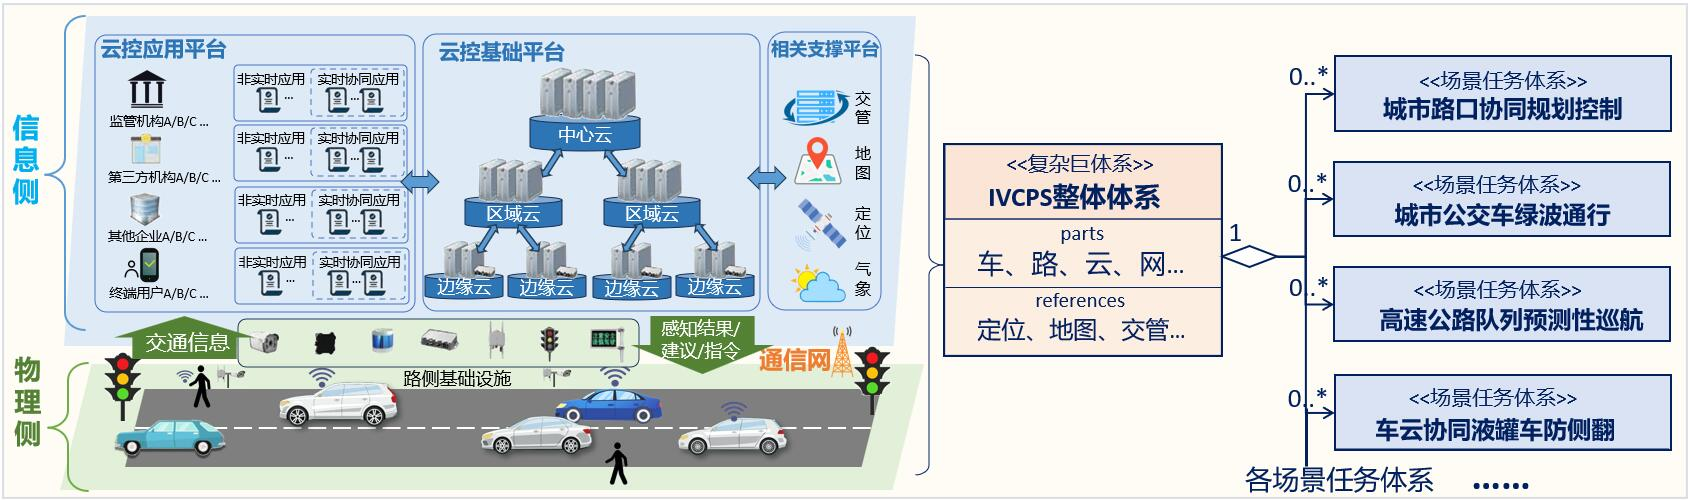
\includegraphics[width=1.0\linewidth]{fig/chap2/sys_consis.jpg}
      \caption{IVCPS整体架构与组成}
      \label{fig:ivcps_sys_consis}
    \end{figure}

    与一般SoS相比，IVCPS对架构建模提出了两个更突出的要求。其一，\emph{场景任务并发}。车路云一体化系统中，智慧公交、智慧环卫、预测性巡航、协同换道、路口协同控制、危化品运输安全保障等多类场景任务可同时发生\cite{caicv2024guideline,lishuyan2022pccheavytrucks,shijia2023cooperativemerging,chenqien2023cpccbus,hans2024}，且共享道路、通信、计算和服务资源，因此架构设计不能只面向单一任务，而必须考虑场景之间的资源竞争与交互影响。其二，\emph{体系持续演进}。随着智能网联车辆渗透率提升、基础设施能力增强和平台服务扩展，IVCPS的协同深度和控制边界会持续变化，同一场景在不同阶段的功能分配和实现方式并不相同。

    体系类型同样影响建模方法选择。现有研究通常根据总体使命与中央管理强弱，将体系划分为虚拟型、协作型、认同型和指向型\cite{fengyimin2024soseframework}。对于IVCPS而言，不同阶段和不同场景往往表现出不同体系类型特征：在低渗透率条件下，由于并非所有车辆均可控，单个场景任务通常更接近认同型体系，系统整体则表现出较强的协作型特征；随着渗透率提高和控制能力增强，部分场景会逐步向指向型体系演化\cite{heqiang2018sosepractice}。因此，IVCPS并不适合采用单一、静态的架构建模方式，而需要能够适应不同阶段、不同场景和不同控制强度的动态建模方法。

    从方法论上看，虚拟型和协作型体系更适合采用基于智能体的建模方法（Agent-based Modeling, ABM）描述成员系统自治行为及其交互涌现\cite{baldwin2015simulation}；指向型体系则更适合采用基于事件的建模方法（Event-based Modeling, EBM），自顶向下描述总体任务、控制逻辑和资源组织\cite{hause2020uafple}。而IVCPS兼具多主体自治、场景并发和中央引导等特征，因此更适合将ABM与EBM结合使用：前者用于反映异构交通参与者的局部决策与群体涌现，后者用于约束关键任务流程、功能分工和安全闭环。基于上述判断构建的IVCPS架构框架矩阵如图~\ref{fig:ivcps_arch_matrix}所示。

    \begin{figure}
      \centering
      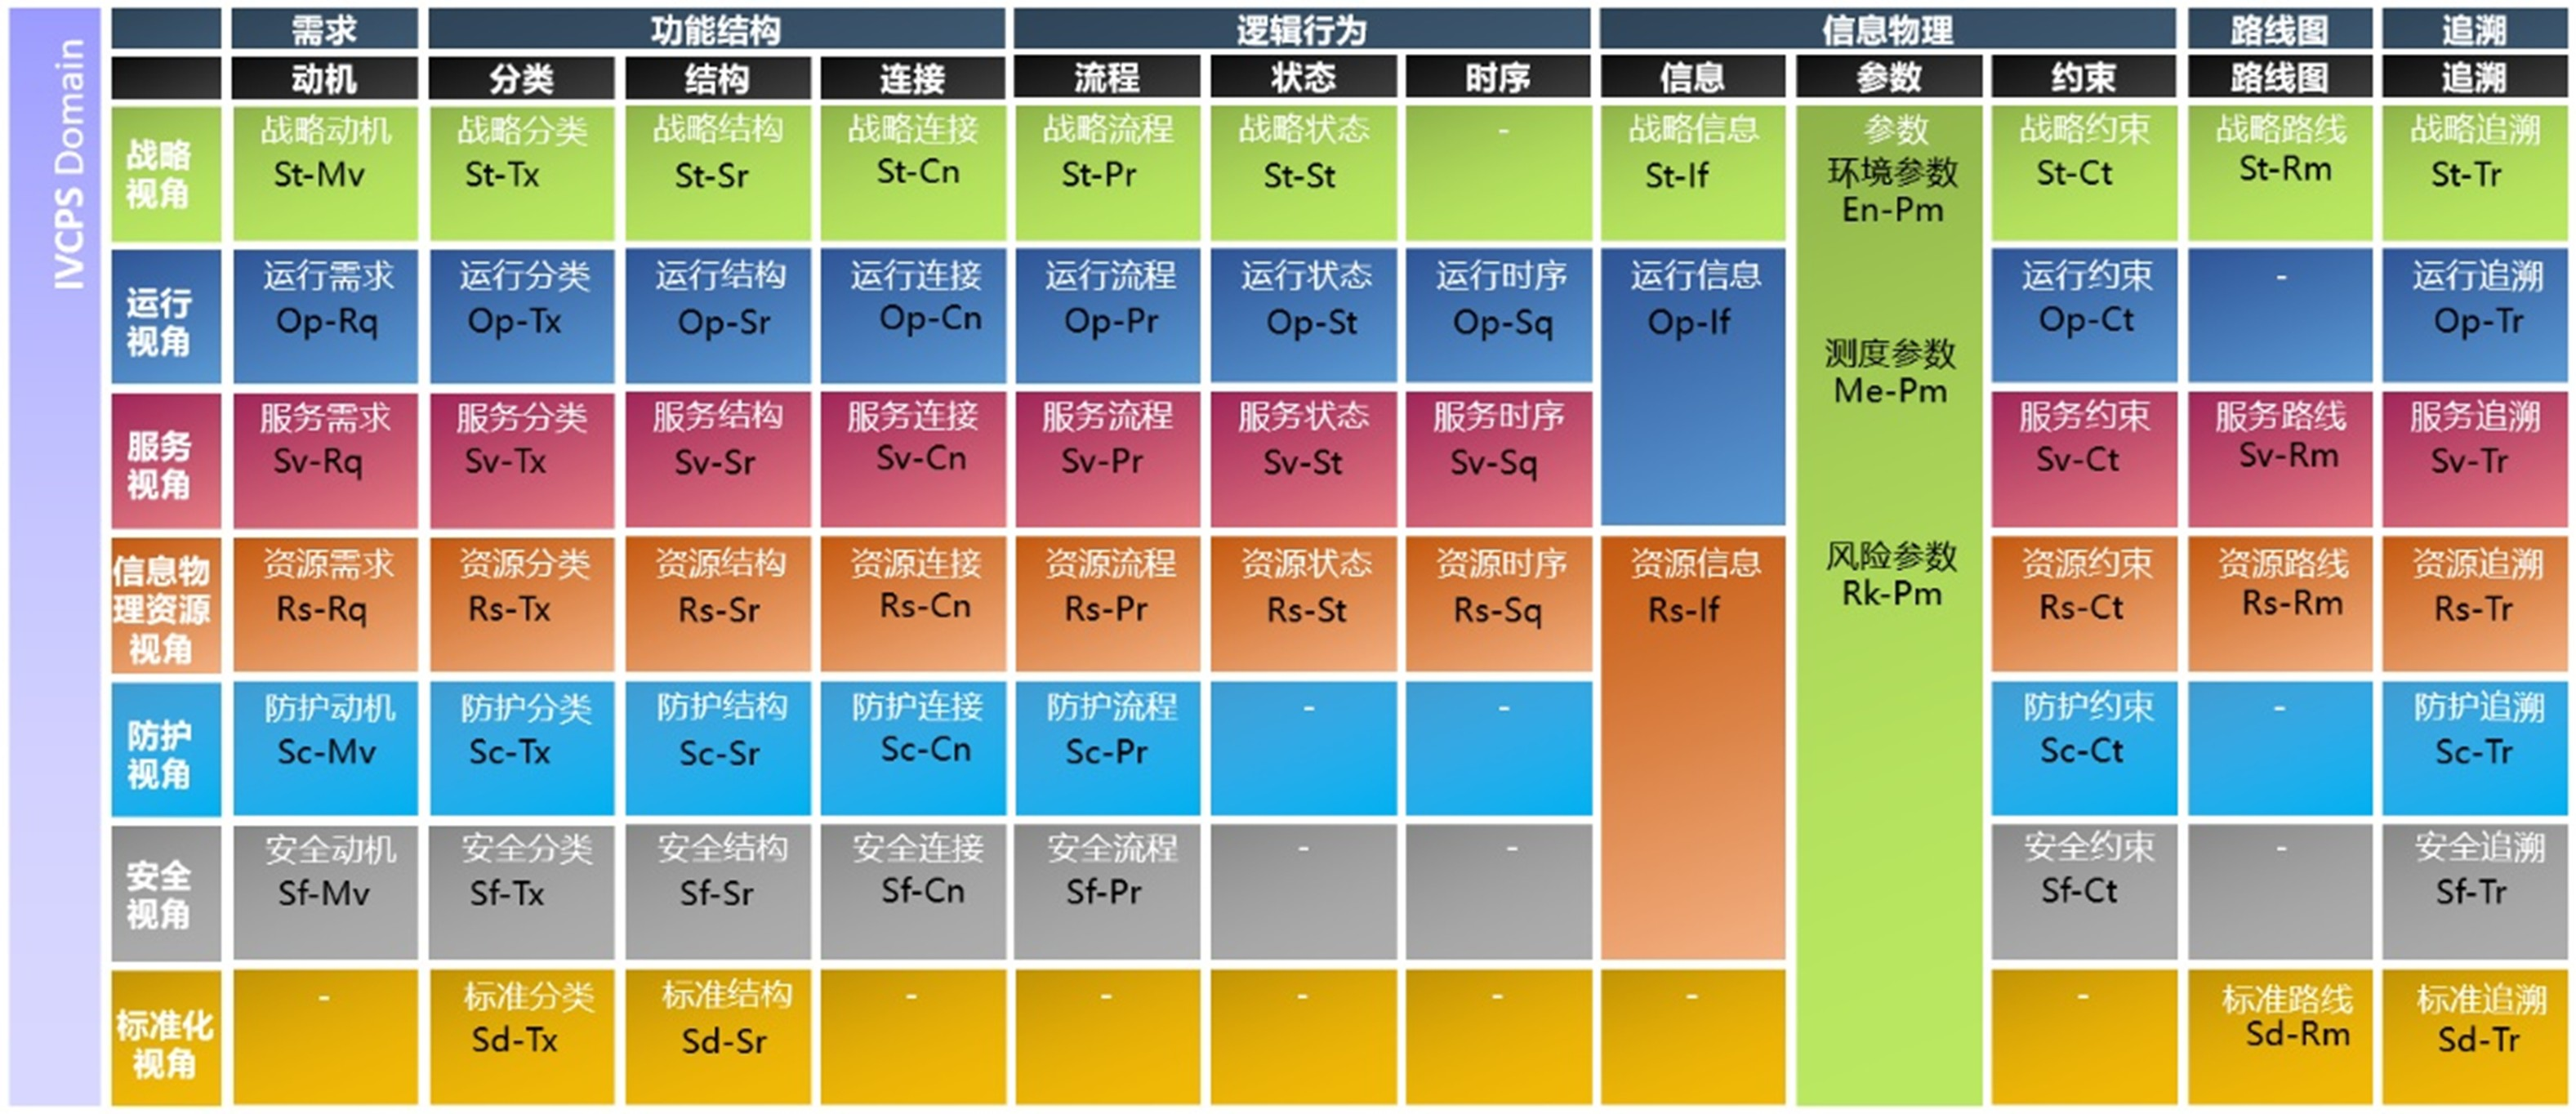
\includegraphics[width=1.0\linewidth]{fig/chap2/ivcps_arch_matrix.jpg}
      \caption{IVCPS架构框架矩阵}
      \label{fig:ivcps_arch_matrix}
    \end{figure}

    对本文研究对象而言，上述特征具有更直接的体现。车云协同液罐车防侧翻任务处于低渗透率高等级公路环境，系统中既存在可控的自动驾驶液罐车，也存在大量不可控的人驾车辆，云端能够提供预测性决策建议，但无法完全替代车端安全闭环。因此，该场景既不是完全分散的协作系统，也不是可由中央全权支配的指向型系统，而是典型的“\emph{局部集中引导 + 车端自主闭环}”体系。这要求建模方法既能描述云端与车端的分工关系，又能通过仿真刻画混合交通流中多主体交互对任务有效性的影响。

    基于上述分析，IVCPS及其场景任务架构建模不宜停留在一次性、静态的系统描述层面，而应采用面向场景任务、能够支撑持续演进与闭环验证的方法。分场景基于模型与仿真的体系工程方法以场景任务为基本构建单元，通过分场景建模、仿真验证和迭代完善逐步形成整体体系架构，能够较好适应IVCPS中“多场景并发、资源共享、持续演进”的特点。对于本文的CT2ROP任务，该方法能够在保持车端、云端和通信链路关系清晰表达的同时，将安全闭环验证纳入架构设计过程，因此更适合作为后续体系架构构建的理论基础。

  \subsection{分场景体系架构建模理论}

    本小节围绕车云协同液罐车防侧翻任务的体系架构设计，说明所采用的建模语言、框架及分场景建模流程。

    \subsubsection*{(1) 建模语言与框架}

      面向复杂体系的架构设计，当前通常以统一架构框架（Unified Architecture Framework, UAF）及其相关扩展为基础，并结合具体领域知识进行裁剪应用\cite{hause2020uafple,hause2021securityviews,hause2021serviceviews,abhaya2021ubm}。其优势在于能够从战略、运行、服务、资源等多个视角统一描述复杂体系中的能力分解、功能协同、资源配置与追踪关系，因此已被广泛用于指挥作战、航空航天和大型信息系统等复杂体系的架构建模\cite{qianqunyou2024uafurbancombat,lvweimin2021dodaf,cuiruijing2025uafindicator,lidelin2024uafcooperation,liminghua2021aerospace,huangran2024lunarserviceuaf,lisong2022uafairtransportation}。

      针对IVCPS这一对象，本文不直接沿用原始UAF，而是结合IVCPS特征与ICV-7S框架，对UAF进行裁剪和重构，形成适用于IVCPS场景任务体系建模的架构框架\cite{qixiaojing2026mbsose,xu2023mbseivcps}。该框架保留了UAF在多视角、一致性和可追踪性方面的优势，同时引入更贴合智能网联汽车系统特点的视角设置。具体而言，框架包含战略、运行、服务、信息物理资源、防护、安全和标准化七个视角，并沿用UAF中动机、分类、结构、连接、流程、状态、时序、信息、参数、约束、路线图和追溯性等方面描述模型元素之间的关系。

      其中，战略视角用于描述体系阶段、能力目标及其演化路径；运行视角用于分析场景任务中的参与方、运行活动及其逻辑关系；服务视角用于将运行活动抽象为可复用、可组合的服务；信息物理资源视角用于描述支撑服务实现的车端、云端、路侧及通信等资源；防护视角和安全视角分别面向信息安全与功能安全/预期功能安全分析；标准化视角则用于约束相关服务和资源的标准依据。相较于原始UAF，该框架更突出IVCPS中安全约束、信息物理融合和场景任务驱动的特点，因此更适合用于本文所研究的CT2ROP任务架构建模。

      在具体实现上，本文采用基于SysML1.5的UAF1.2元模型对裁剪后的IVCPS架构框架进行表达，并在此基础上扩展安全视角相关元素，用于后续架构模型建立与分析。面向IVCPS的分场景体系架构建模流程如图~\ref{fig:ivcps_time_series}所示。

      \begin{figure}[htbp]
        \centering
        \makebox[\linewidth]{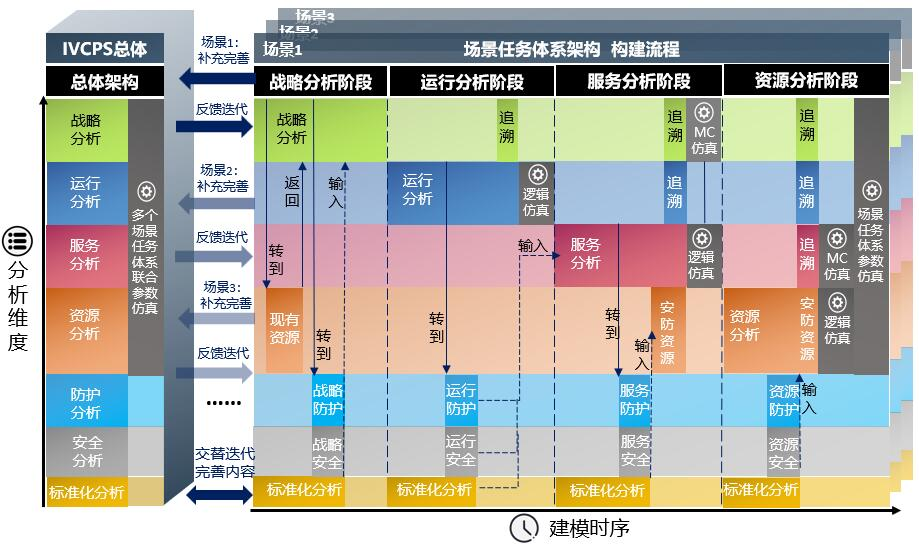
\includegraphics[width=1.0\linewidth]{fig/chap2/time_series.jpg}}
        \caption{面向IVCPS的分场景体系架构建模方法流程分视角时序拆解示意}
        \label{fig:ivcps_time_series}
      \end{figure}

    \subsubsection*{(2) 总体流程思路概述}

      面向IVCPS这类开放演进的CPSoS，本文提出分场景基于模型与仿真的体系工程（scenario-oriented model and simulation based system-of-systems engineering, So-MBSoSE）方法\cite{qixiaojing2026mbsose}。该方法以场景任务为基本构建单元，通过场景迭代不断完善整体架构、识别跨场景交互，并将建模、仿真与验证纳入统一闭环。相较于一次性、自上而下的静态架构描述，这种方法更适合处理IVCPS中场景持续扩展、多主体协同以及安全闭环需反复验证的特点，也更契合CT2ROP这类需要同时统筹车端、云端、通信链路与安全约束的复杂任务。

      本文采用面向场景任务的分场景体系建模思路。其基本思想是：将IVCPS整体架构视为多个场景任务体系架构的综合，各场景任务在共享统一框架的前提下分别建模、分别验证，并在迭代过程中不断补充和完善整体架构。对于本文关注的CT2ROP任务，即先建立液罐车防侧翻场景任务体系架构，再通过与整体IVCPS架构的映射关系明确其在系统中的功能定位、接口关系与资源依赖。

      单个场景任务体系架构设计总体分为四个阶段：战略分析阶段、运行分析阶段、服务分析阶段和资源分析阶段。战略分析阶段从任务使命、能力目标与发展约束出发，明确场景任务要解决什么问题以及能力如何分层落实；运行分析阶段面向参与主体与运行活动，构建可行的运行方案并梳理活动逻辑；服务分析阶段将运行活动进一步抽象为服务，以实现运行层与资源层之间的解耦，提高架构的可复用性和适应演进能力；资源分析阶段则进一步落实支撑服务实现所需的信息、通信、计算和物理资源，为后续具体实现提供依据。

      安全、防护和标准化分析贯穿上述四个阶段。战略阶段形成总体约束，运行阶段识别任务执行过程中的安全与防护需求，服务阶段落实相关服务分类与接口规范，资源阶段则进一步将这些要求细化到具体资源配置与实现约束中。这样可使安全、防护和标准要求不再作为附加分析，而是嵌入到体系架构设计全过程之中。

      从方法论上看，该流程同时体现了自顶向下和自底向上的结合。四阶段逐层分解体现了基于事件的建模思想，即从任务目标出发逐步落实到活动、服务和资源；而仿真验证则体现了基于智能体和系统交互涌现的思想，通过仿真反馈不断修正架构设计。为此，本文在不同阶段引入了不同层次的验证活动：运行分析阶段主要验证运行逻辑是否闭合；服务与资源分析阶段引入逻辑仿真和Monte Carlo仿真，以分析指标、参数与能力测度之间的一致性；资源阶段进一步开展场景任务体系参数仿真，从体系层面对架构设计的合理性进行初步检验。


\section{车云协同液罐车防侧翻行驶架构建模}

本节以图~\ref{fig:ivcps_time_series}所示的分场景体系架构建模流程为指导，构建车云协同液罐车防侧翻/危化品运输（Cloud-based tank truck rollover prevention, CT2ROP）场景任务体系架构。本节的分析主线为：战略阶段确定场景边界、风险结构、能力目标与总体分工，运行阶段确定主体职责与协同关系，服务阶段将运行活动抽象为可约束、可验证的服务并给出参数边界，资源阶段落实支撑服务实现的软硬件基础与场景级参数来源，就此形成了完整的架构设计流程结果图\cite{KomasaQi2026MasterThesis_repo}。

  \subsection{CT2ROP架构概览}

    CT2ROP是IVCPS在低渗透率高等级公路环境下面向危化品运输主动安全保障的典型场景任务。本场景中，液罐车运行风险同时受道路几何、周车行为、液体晃动和通信状态影响，相关安全能力由车端、云端、路侧及相关平台共同提供。CT2ROP场景概念架构如图~\ref{fig:ct2rop_concept}所示。

    \begin{figure}
      \centering
      \makebox[\linewidth]{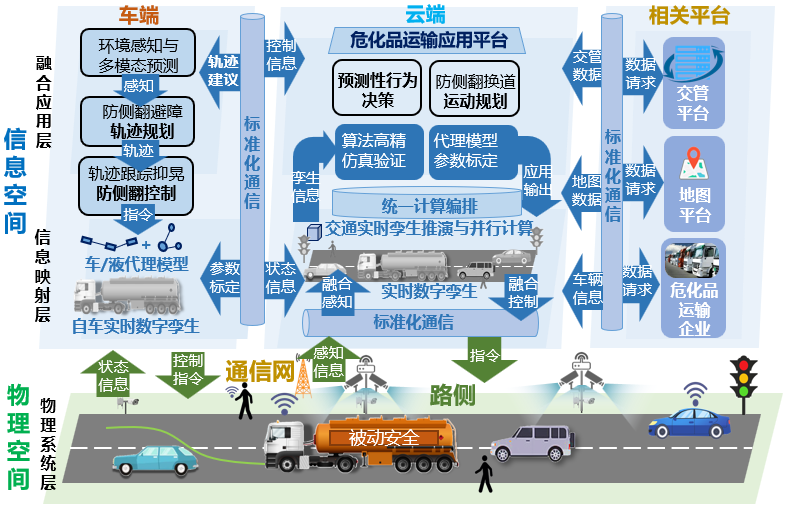
\includegraphics[width=0.8\linewidth]{fig/chap2/ct2rop_concept.png}}
      \caption{车云协同危化品运输场景概念架构}
      \label{fig:ct2rop_concept}
    \end{figure}

    CT2ROP总体上由车端、云端、路侧和相关平台共同构成。车端承担局部环境感知、防侧翻轨迹重规划与实时控制，云端承担交通孪生、预测性行为决策与防侧翻换道运动规划，路侧设备负责结构化交通环境感知，地图平台、交管平台和危化品运输企业平台分别提供静态环境、准静态交通管理信息以及运输业务支撑。CT2ROP中的状态获取、风险预测、决策生成与控制执行分布于不同主体之中，需通过体系架构完成功能组织与边界划分。在该概念架构基础上，结合后续战略、运行、服务和资源分析结果，本节进一步形成图~\ref{fig:safe_arch}所示的分层决控架构。

    \begin{figure}[htbp]
      \centering
      \makebox[\linewidth]{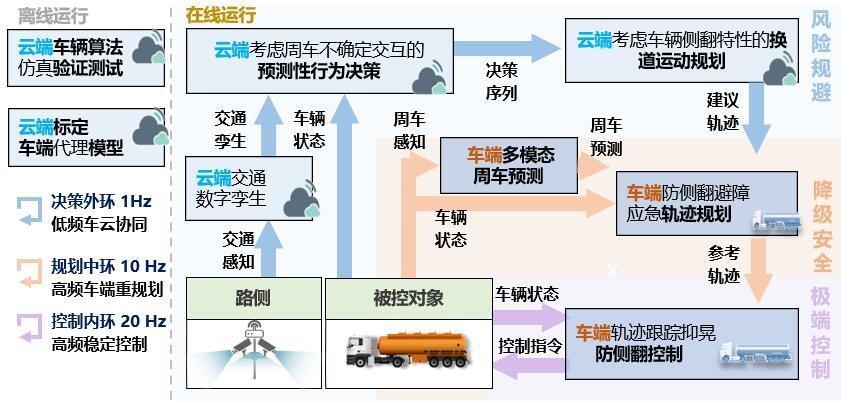
\includegraphics[width=1.0\linewidth]{fig/chap2/safe_arch.jpg}}
      \caption{车云协同液罐车防侧翻分层决控架构}
      \label{fig:safe_arch}
    \end{figure}

    该架构由云端低频决策外环、车端中频规划中环和车端高频控制内环构成，对应风险规避、降级安全和极端控制三层任务。该分层反映三类功能在信息范围、可容许时延和被控对象动态时间尺度方面的差异：云端面向更大空间范围的交通状态和更长时域的风险演化，车端规划层直接面向局部环境与可行轨迹生成，车端控制层直接作用于执行器并抑制快速动态风险。围绕上述目标架构，本节进一步按战略、运行、服务和资源四阶段开展CT2ROP场景任务体系架构设计，并在各阶段中给出对后续章节具有约束作用的结论。



  \subsection{CT2ROP架构详细设计}
  \label{sub:ct2rop_arch_detail}

    本小节围绕战略、运行、服务和资源四个阶段展开CT2ROP场景任务体系架构设计，分析各阶段输入输出及图~\ref{fig:safe_arch}所示分层决控架构关系在所推导约束下的形成过程。

    \subsubsection{场景战略分析}

      战略分析阶段的输入主要包括三类内容：其一，CT2ROP场景在IVCPS中的演进阶段；其二，现有资源基础及其阶段性继承关系；其三，危化品运输事故特征、风险链条及相应安全目标。围绕这三类输入，本小节依次分析体系阶段、资源条件、风险结构与能力需求。其中，CT2ROP战略演进阶段如图~\ref{fig:stage}所示。

      \begin{figure}
        \centering
        \makebox[\linewidth]{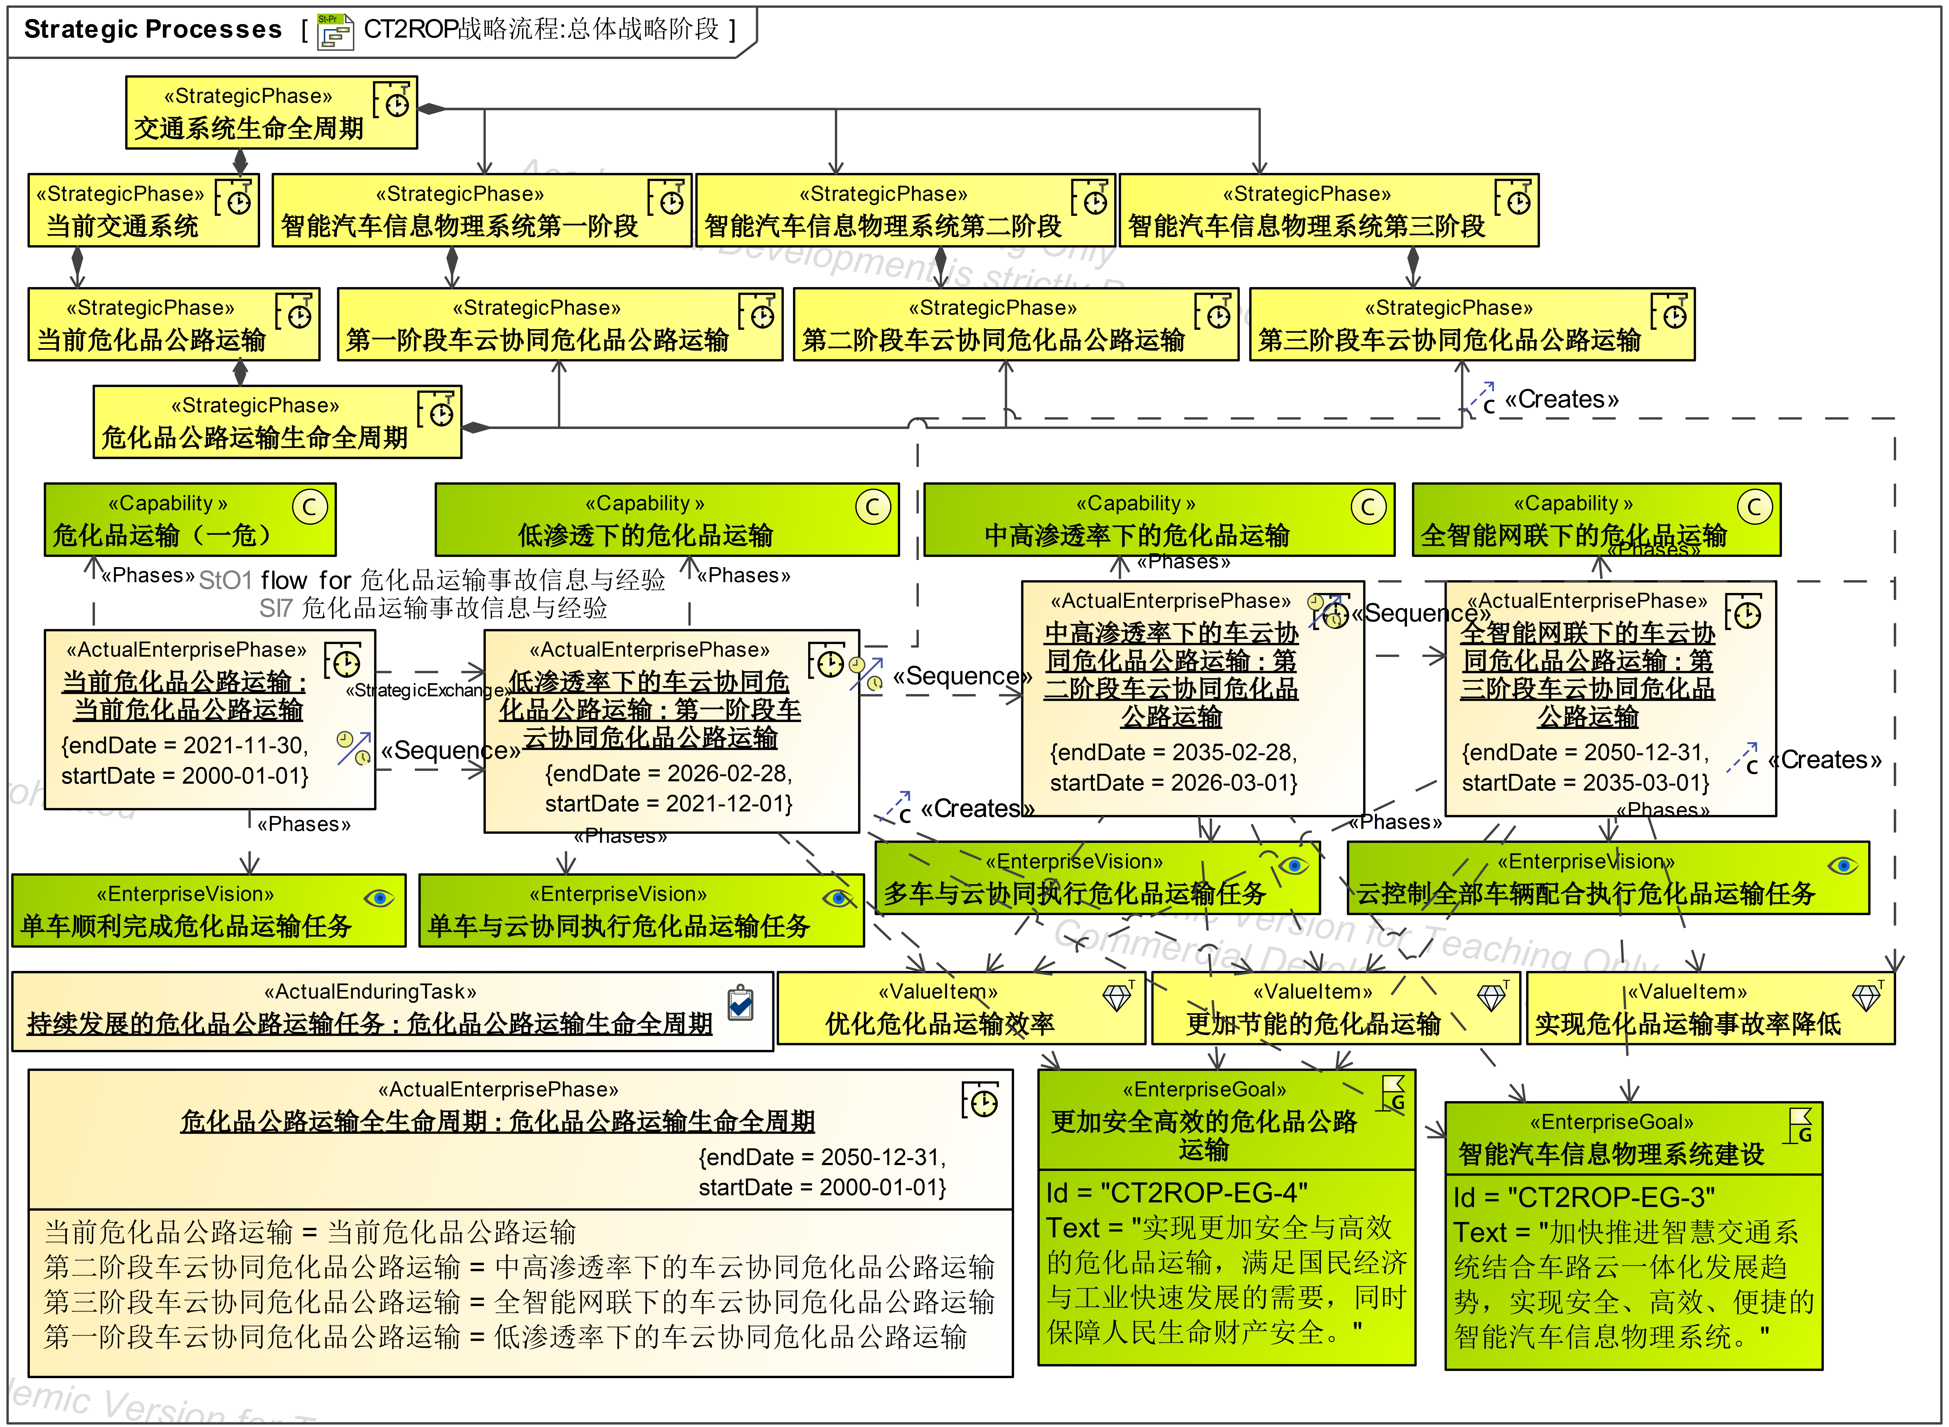
\includegraphics[width=1.0\linewidth]{fig/chap2/stage.png}}
        \caption{CT2ROP战略演进阶段}
        \label{fig:stage}
      \end{figure}

      首先，从体系演进阶段看，CT2ROP场景作为IVCPS的重要组成部分之一，遵循与IVCPS一致的演化路径，从当前阶段逐步经历低渗透率、中高渗透率直至全智能网联阶段。图中各阶段能力目标和任务形态的变化表明，CT2ROP所依托的体系能力随智能网联车辆渗透率提升而逐步增强。当前研究对象处于低渗透率阶段，交通系统中仍存在大量不可控车辆，路侧和云端能力覆盖有限，云端建议的可执行性受车端状态、通信链路和局部环境共同制约。由此，后续架构设计需以“部分可控、混合交通、局部兜底”为基本前提。CT2ROP资源分类与结构如图~\ref{fig:resource_model}所示。

      \begin{figure}
        \centering
        \makebox[\linewidth]{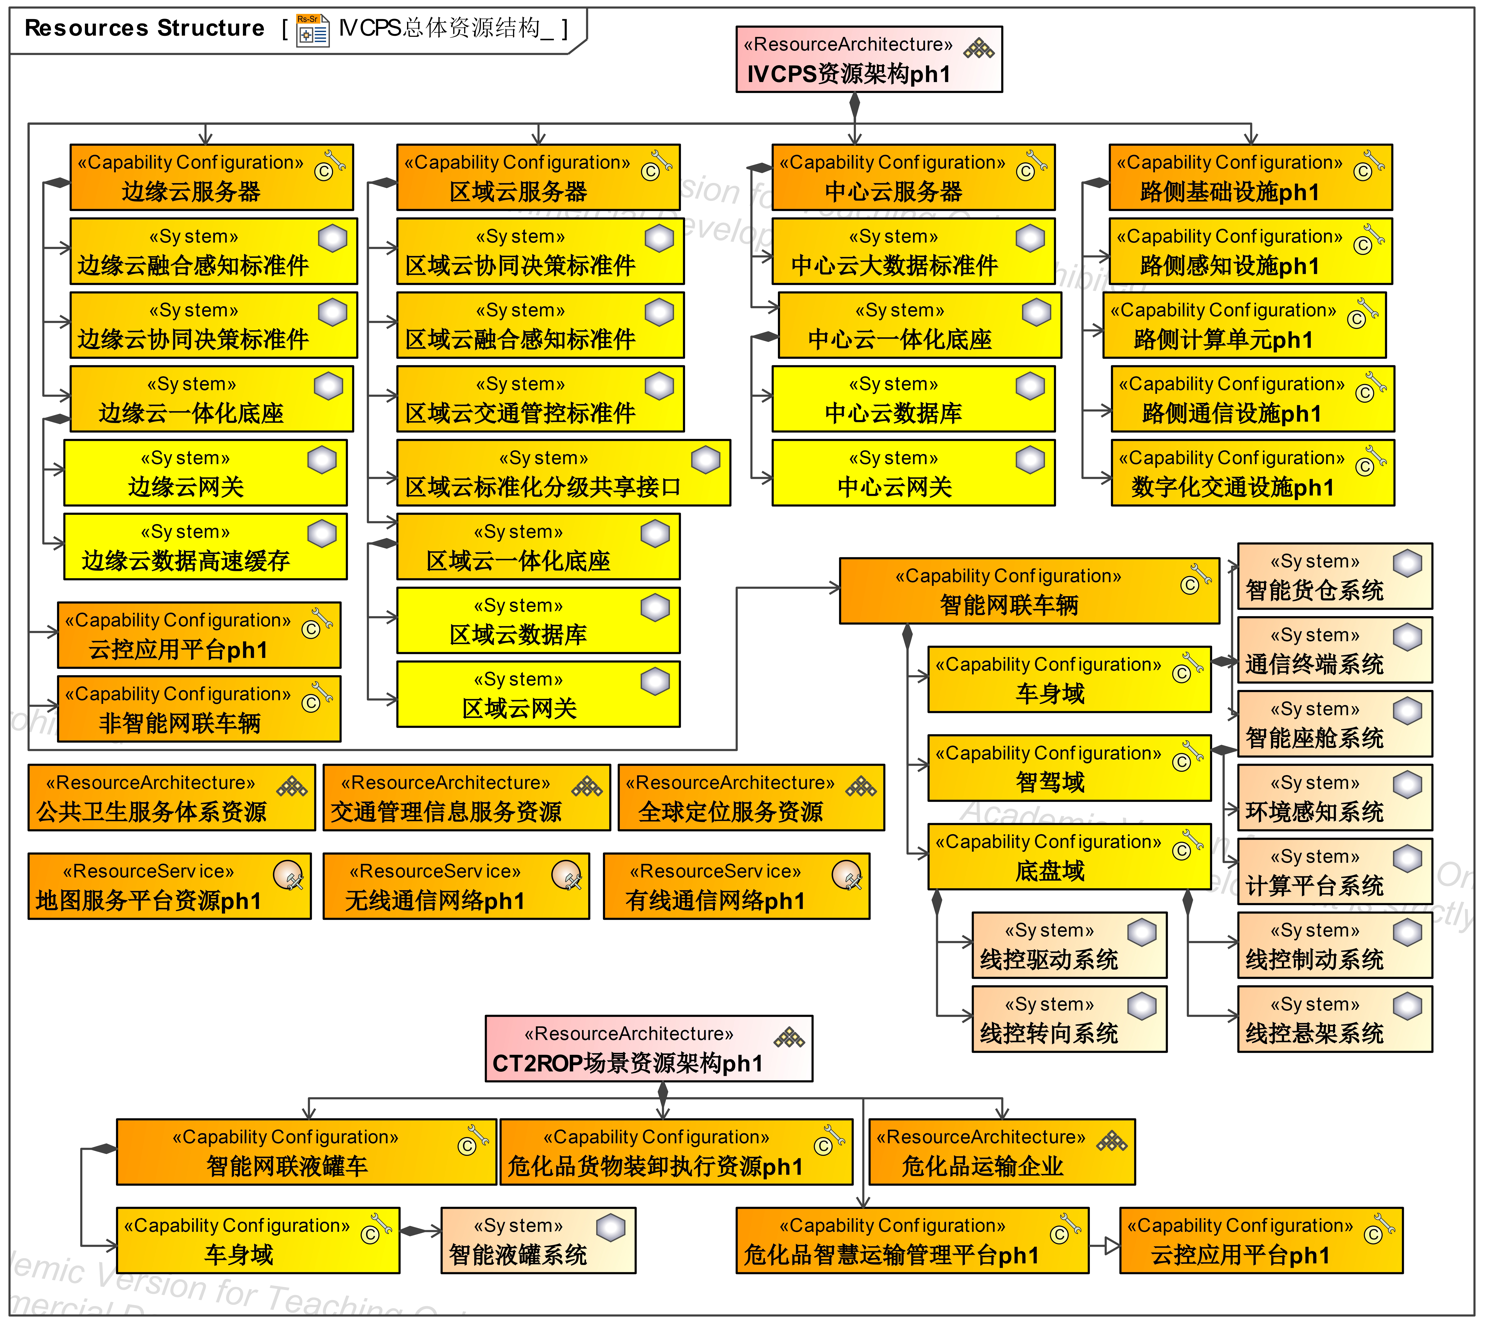
\includegraphics[width=1.0\linewidth]{fig/chap2/resource_model.png}}
        \caption{CT2ROP资源分类与结构}
        \label{fig:resource_model}
      \end{figure}

      其次，从资源基础看，CT2ROP场景任务建立在IVCPS总体资源体系之上，主要包括智能车辆、云控基础平台与应用平台、路侧基础设施以及交管、地图等支撑平台。云端与路侧设施为多场景共享资源，共同构成数据采集与计算基础；液罐车、危化品运输平台等则属于CT2ROP场景特有资源。该资源结构表明，云端预测与路侧感知能力具有共享资源受限特征，车端规划与控制能力则需在场景特有资源中得到落实。由此，关键安全能力需在车端形成独立闭环，云端和路侧能力用于扩展感知范围和前移风险规避能力。

      在战略环境分析方面，结合现有事故资料可知，液罐车危化品运输事故在山东、江苏、浙江等地区较为集中，高速公路和一级公路是主要发生道路类型，出入口匝道、下坡转弯、城市交叉口、桥梁涵洞和收费站等特殊路段风险更高；在事故诱因方面，侧翻与碰撞追尾最为常见，液化石油气、液化天然气、汽柴油等介质风险突出，且半载工况下侧翻风险显著增大，后续章节仿真验证场景设置将参考上述分析。



      基于事故相关的场景分析，本小节将运输过程中的风险按照事故逻辑链位置划分为四类：根源性风险、诱发性风险、状态性风险和后果性风险。根源性风险对应设计、管理和人员等基础层面缺陷，是其他风险的底层诱因；诱发性风险对应运输过程中的外部扰动、操作失误、协同链路异常等，其中液体晃动是液罐车特有且具有直接诱发作用的关键因素；状态性风险对应车辆、罐体和车云协同链路进入异常状态而尚未完全演化为事故的阶段；后果性风险则对应事故发生后的最终损失与次生灾害。不同位置风险即可对应不同控制时机与处置逻辑：根源性风险对应源头防控，诱发性风险对应过程预警，状态性风险对应实时干预，后果性风险对应应急处置。

      在上述阶段、资源和风险分析基础上，如图~\ref{fig:safe_capability}所示，本小节进一步提炼出危化品公路运输主动安全保障所需的四类核心能力：态势感知与风险识别、风险预测与预防性干预、风险控制与稳定性保障、鲁棒性与安全运营。CT2ROP同时面临多源异构信息输入、液体晃动引发的状态演化以及通信不确定性，因此首先需要态势感知与风险识别能力；诱发性风险在进入危险状态前具有可观测和可预测特征，因此需要风险预测与预防性干预能力；低渗透率条件下云端干预始终存在时延与失效可能，体系需具备局部实时可行运动规划与极限稳定保持能力，因此需要风险控制与稳定性保障能力；通信、感知和服务可用性随任务过程变化，体系需在退化条件下维持安全运行和可追溯性，因此需要鲁棒性与安全运营能力。图中的能力、测度指标与战略约束之间建立了后续运行、服务和资源分析的追溯关系。

      战略阶段的分析由此形成三项架构约束。其一，低渗透率条件下的CT2ROP需采用云端与车端协同分工的总体架构，因为阶段分析表明云端能力存在范围与可控性边界，资源分析表明共享外部资源不承担全部关键安全职责。其二，风险处置需采用分层组织方式，因为风险链条本身具有“根源—诱发—状态—后果”的演化顺序，不同风险位置对应不同控制时机。其三，后续方法设计需围绕四类核心能力及其测度展开，其中云端主要支撑态势感知、风险预测与预防性干预，车端主要支撑风险控制与稳定性保障，并共同支撑鲁棒性与安全运营。

     \begin{figure}
        \centering
        \makebox[\linewidth]{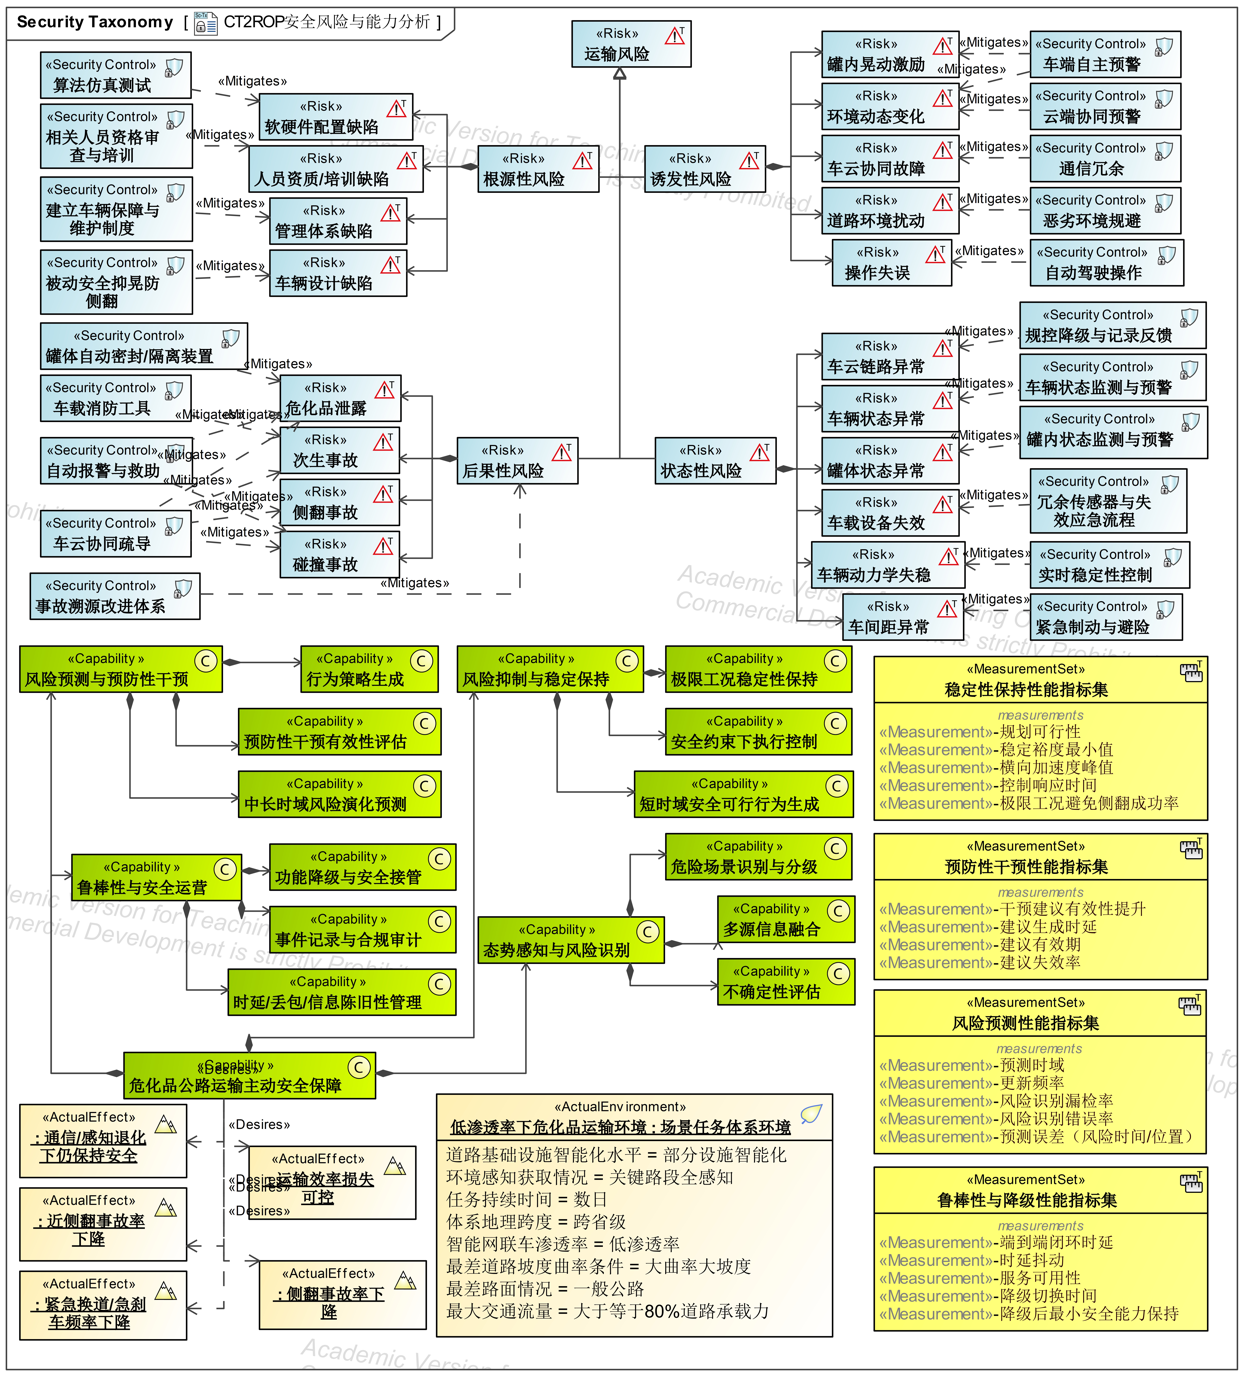
\includegraphics[width=1.0\linewidth]{fig/chap2/safe_capability.png}}
        \caption{CT2ROP安全与能力分析}
        \label{fig:safe_capability}
      \end{figure}
 

    \subsubsection{场景运行分析}

      运行分析阶段的输入来自战略阶段形成的能力目标、风险处置逻辑和环境约束。运行分析的任务，是将这些较高层级的能力要求落实为可执行的运行主体、运行活动及其交互关系，从而判断各主体在任务执行过程中的职责划分是否能够支撑前述战略能力。

      根据前述四类核心能力，CT2ROP可首先抽象为运营监管、道路基础设施、协同支撑和运输车辆四类运行执行者。结合资源结构，进一步可具象化为危化品运输指挥与控制平台、路侧智能设施、边缘云及地图/交管支撑平台、智能网联液罐车等关键运行主体，如图~\ref{fig:operation_model}所示。图中不同执行者之间的连接关系表明，CT2ROP运行涉及运输任务管理、环境感知、信息融合和车辆执行等多个环节。由此，后续方法设计中的“车端/云端/平台”划分首先服从运行主体的职责划分。

      \begin{figure}
        \centering
        \makebox[\linewidth]{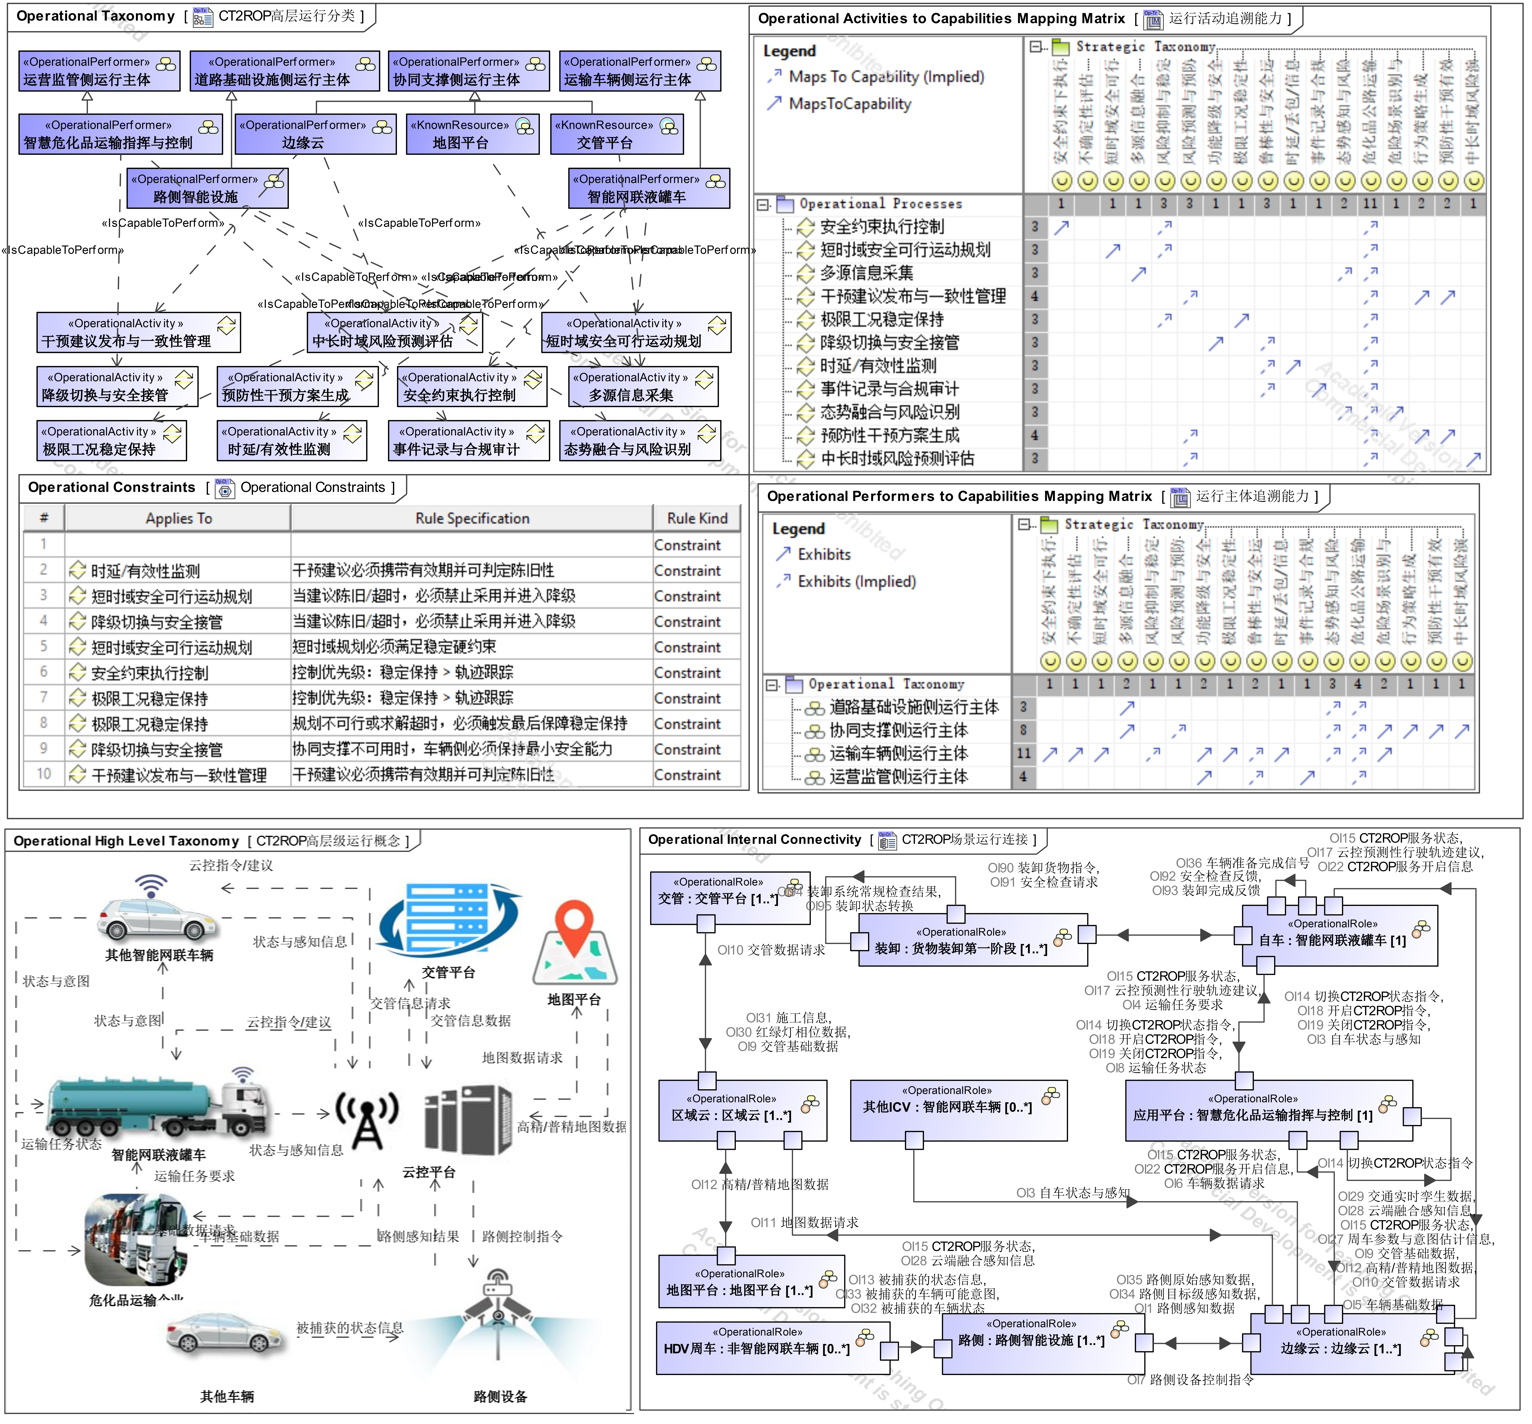
\includegraphics[width=1.0\linewidth]{fig/chap2/operation_model.png}}
        \caption{CT2ROP运行分类及结构分析}
        \label{fig:operation_model}
      \end{figure}

      危化品运输指挥与控制平台负责运输任务创建、阶段切换与业务监管，属于静态调度主体；边缘云和云控平台负责基于路侧感知、车端上报以及平台信息开展交通孪生与预测性引导，属于低频协同支撑主体；智能网联液罐车负责局部环境感知、执行规划和实时控制，属于高频任务执行主体。上述分工成立的原因在于各主体所掌握的信息范围、可允许的处理时延和直接作用对象不同：平台掌握运输任务和业务上下文，云端掌握更大空间范围的信息并具备较强计算资源，车端最接近执行器与局部环境。

      运行层逻辑仿真进一步用于验证上述运行分工在过程层面是否闭合。CT2ROP运行功能与逻辑仿真实现了运行活动在单车模式与协同模式之间的切换逻辑、运输任务创建与结束过程，以及运行执行者之间的主要信号交互等\cite{KomasaQi2026MasterThesis_repo}。

      运行阶段由此明确了后续服务层的基础关系：运营监管侧、道路基础设施侧、协同支撑侧及运输车辆侧4大运行主体为核心执行者；体系中的信息流遵循“车端上传状态与感知信息—云端融合并生成建议—车端执行、拒绝或降级接管”的基本模式；车端在运行逻辑中承担独立安全执行职责。后续服务层即围绕上述交互关系定义接口、触发条件和降级规则，形成图~\ref{fig:service_definition}所示的服务约束视图。

      \begin{figure}[htbp]
        \centering
        \makebox[\linewidth]{\includegraphics[width=1.0\linewidth]{fig/chap2/service_definition.png}}
        \caption{服务约束视图下定义的CT2ROP专有服务及IVCPS通用服务}
        \label{fig:service_definition}
      \end{figure}

   

    \subsubsection{场景服务分析}

      服务分析阶段的输入包括运行阶段形成的主体交互关系和战略阶段给出的能力测度。其任务是将运行活动抽象为可复用、可约束和可追溯的服务，并进一步确定这些服务的接口、更新周期、时延约束和降级规则。

      细化服务约束后的服务定义总结了不同场景任务中的共性服务与CT2ROP场景中的特有服务\cite{KomasaQi2026MasterThesis_repo}。IVCPS总体中已存在路侧感知信息提供、地图信息提供、车云通信等多运行场景可复用的共性服务；在此基础上，CT2ROP场景形成了危化品运输车辆任务调度、云端预测性轨迹规划、车端防侧翻规划与控制以及液罐车装卸载等场景特有服务。服务层的关键作用在于解耦运行逻辑与资源实现：运行层围绕服务接口组织活动，资源层围绕服务约束提供实现基础，由此使架构能够适应阶段演进和资源更新。CT2ROP服务功能与逻辑相比运行层被更加精细地进行仿真\cite{KomasaQi2026MasterThesis_repo}以明确服务之间的调用顺序、服务内部子服务的协同过程以及服务架构内部的信息交互关系。由此，后续章节中云端决策、车端规划和车端控制的输入、输出、触发与反馈关系均可追溯到图~\ref{fig:service_trace}所示的服务层定义。


      \begin{figure}[htbp]
        \centering
        \makebox[\linewidth]{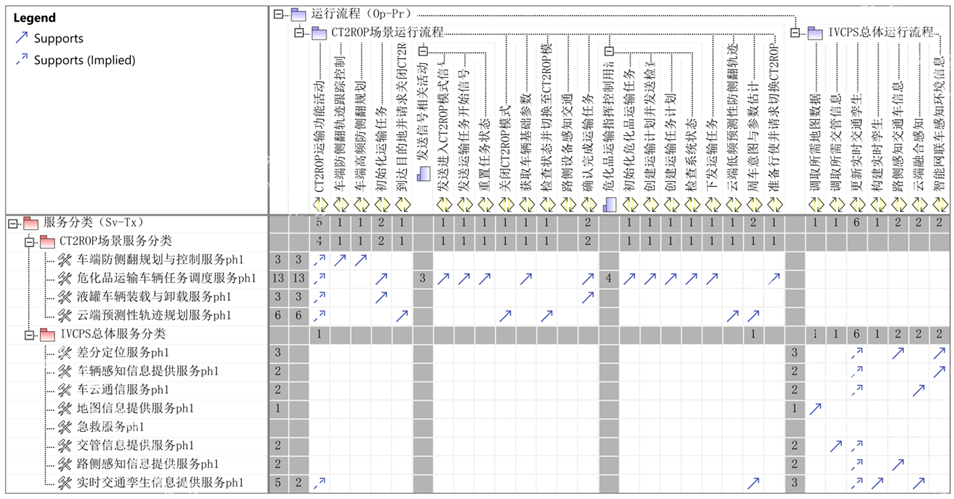
\includegraphics[width=1.0\linewidth]{fig/chap2/service_trace.png}}
        \caption{所有服务与运行活动间的追溯关系}
        \label{fig:service_trace}
      \end{figure}

      服务阶段更关键的工作在于参数级分析，即调整服务参数使得服务规范满足战略能力中的关键测度要求。如图~\ref{fig:service_time_sim}所示，“低渗透率下的危化品运输”战略能力中的应急响应时间指标描述从危险被感知到相应决策与规划被执行器执行的总时延，受车端感知、路端感知、车端规划、云端规划、车云通信和路云通信等多个服务参数共同影响，属于服务层必须验证的综合性指标。在仿真实现中，战略约束层中关于应急响应时间的约束被作为蒙特卡洛（Monte Carlo, MC）仿真的检验标准。参数图描述了从各相关服务中提取服务规范参数、输入MATLAB进行实际测度计算、返回实际测度并与战略约束进行比对的过程。通过每轮1000次的MC仿真迭代，服务规范参数被逐步调整，使仿真结果的均值和超调比例同时满足要求。参数调整要求必须存在车端独立应急响应链路以保证将平均应急响应时间压缩到\SI{100}{ms}量级之内。

      \begin{figure}
        \centering
        \makebox[\linewidth]{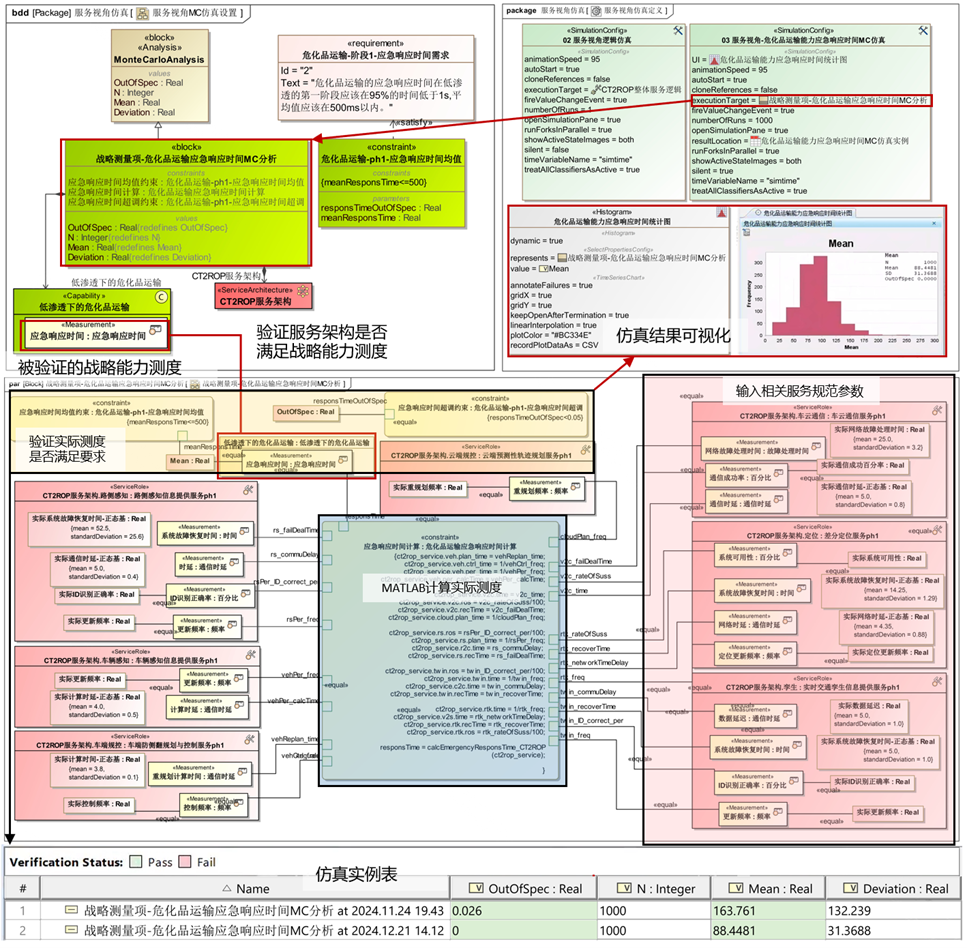
\includegraphics[width=1.0\linewidth]{fig/chap2/servie_time_sim.png}}
        \caption{服务阶段应急响应时间蒙特卡洛仿真}
        \label{fig:service_time_sim}
      \end{figure}



      任务时间尺度同样推导自稳定性仿真。从控制理论角度看，CT2ROP中的云端决策层、车端规划层和车端控制层均可视作闭环系统。闭环控制周期需显著小于所关注任务的主导动态时间尺度，否则系统稳定性难以保障；同时基于模型的控制方案需保证推演时域大于等于主导动态时间尺度。结合服务层参数分析与现有车云协同研究中关于通信时延、抖动和丢包的结论\cite{xionglu2024_CVIS_survay,xuqing2021unreliable,wang2021platoonmpc}，可以将CT2ROP中的典型任务划分为三类时间尺度：车辆纵向速度渐进调整和巡航速度优化属于\SIrange{5}{10}{s}量级慢变量任务；换道和局部避障属于\SIrange{4}{6}{s}量级行为与轨迹重构任务；轨迹跟踪、侧倾抑制和液体晃动耦合稳定控制属于更快的稳定性相关任务，其中液体晃动主导周期约为\SI{1.5}{s}量级。CT2ROP服务功能与逻辑仿真如图~\ref{fig:service_sim}所示。

      \begin{figure}[h!]
        \centering 
        \makebox[\linewidth]{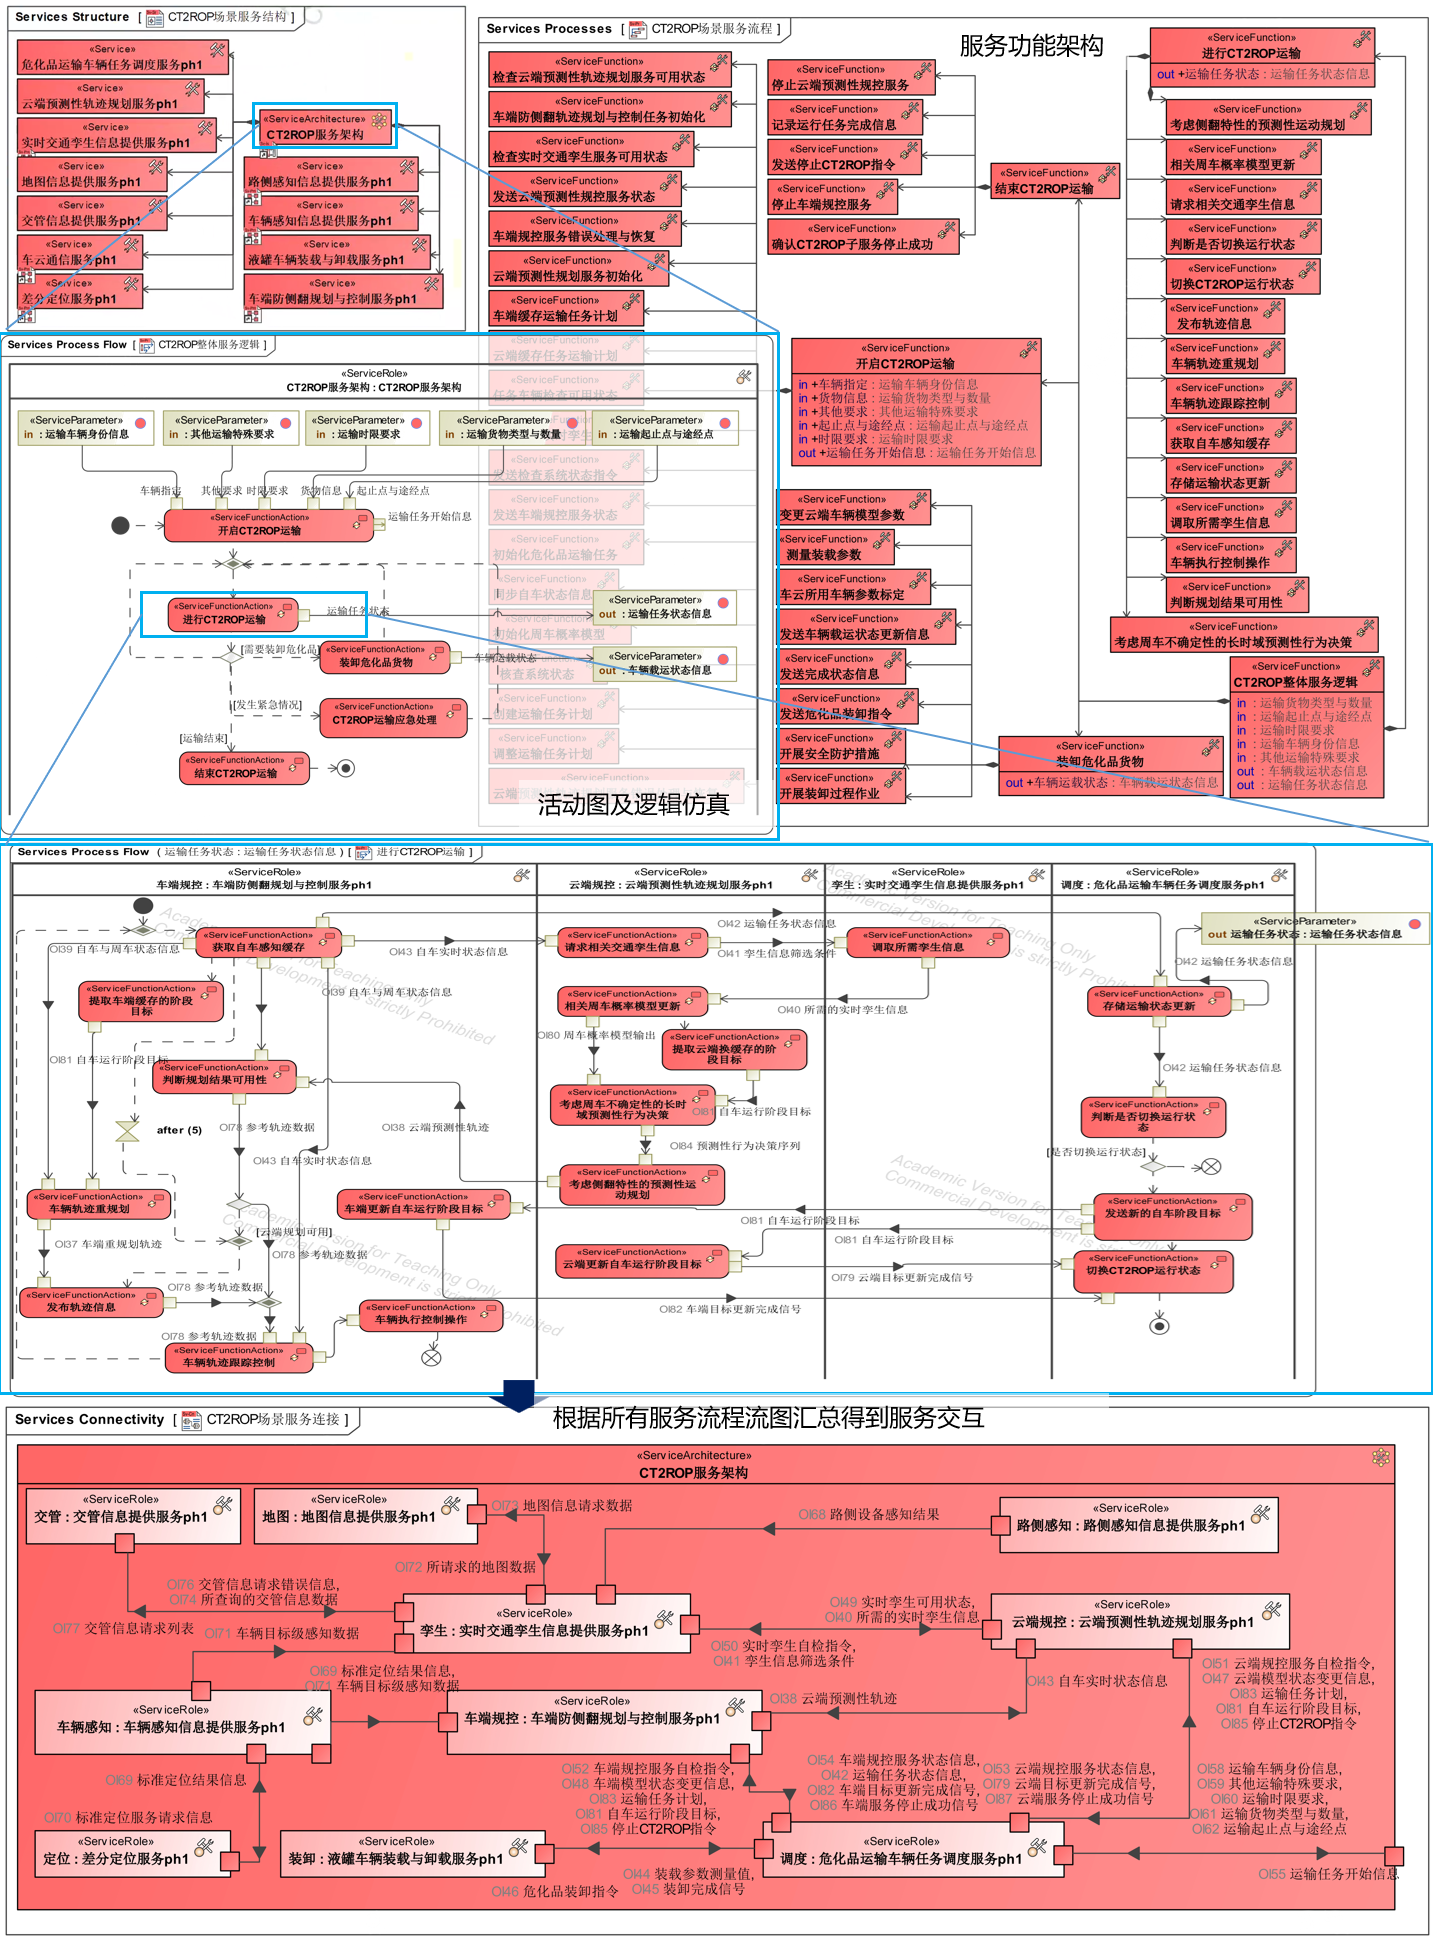
\includegraphics[width=1.0\linewidth]{fig/chap2/service_sim.png}}
        % \caption*{图片注释解释说明}
        \caption{CT2ROP服务功能与逻辑及其仿真}
        \label{fig:service_sim}
      \end{figure} 


      在上述时间尺度背景下，服务参数分析进一步给出分层服务周期。云端链路包含状态上传、融合计算、建议生成和下发执行等多个环节，受通信时延和尾部波动影响，其更新频率适合落在\SIrange{1}{2}{Hz}量级；该频率能够支撑\SIrange{5}{10}{s}量级纵向速度调整与\SIrange{4}{6}{s}量级换道引导，因此云端服务适合承担长时域预测性决策和参考轨迹生成，推演时域应保证\SIrange{10}{30}{s}。车端规划层直接面向局部环境和执行约束，感知到规划的闭环路径更短，因此其更新频率需提升到\SI{10}{Hz}量级，以保证在局部扰动、障碍出现或云端建议变化时能够及时重构轨迹，规划时域满足\SI{5}{10}{s}。车端控制层直接作用于执行器，并需应对\SI{1.5}{s}量级液体晃动和车辆横摆/侧倾耦合动态，因此控制闭环需进一步提升到\SI{20}{Hz}及以上，使控制周期相对于主导动态保持足够小的比例，并保证至少\SIrange{2}{3}{s}的预测时域确保覆盖液体完整动态。



      由此，服务阶段形成了对图~\ref{fig:safe_arch}中时间尺度分层的直接支撑：关键安全链路由车端本地闭环主导，云端承担预测性辅助；云端、车端规划层和车端控制层分别对应\SI{1}{Hz}、\SI{10}{Hz}和\SI{20}{Hz}量级的服务周期；服务接口中需显式定义云端建议的超时判定、失效处理和车端降级接管机制，以保证在通信尾部时延或服务不可用条件下仍满足战略能力中的应急响应要求。




    \subsubsection{场景资源分析}
      \label{subsubsec:resource_analysis}

      资源分析阶段的输入包括服务阶段形成的服务接口、性能约束和更新周期。其任务是将这些抽象约束落实为具体软硬件资源，并进一步验证这些资源是否足以支撑前述服务规范与战略能力。

      如图~\ref{fig:safety_model}所示，资源分析在IVCPS总体资源结构基础上，对CT2ROP场景特有资源进行补全。围绕战略阶段给出的主动安全控制需求和服务阶段给出的时间尺度约束，本小节进一步归纳出六类关键资源：算法仿真测试资源、车端自主预警资源、车云协同预警资源、规控降级与记录反馈资源、紧急制动与避险资源、实时稳定控制资源。云端长时域推演对应高保真液罐车动力学仿真模型、典型工况库和预测性决策程序；车端自主预警对应智能液罐系统、车载通信终端和状态监测资源；车端中高频规划与控制对应车端防侧翻避障规划程序、轨迹跟踪抑晃防侧翻控制程序和本地计算平台。

      资源分析通过相比运行与服务更加详细的逻辑仿真、资源参数级MC仿真以及场景级参数仿真进一步验证资源配置能否支撑服务层定义的性能要求\cite{KomasaQi2026MasterThesis_repo}。其中逻辑仿真用于检验资源实现服务的过程逻辑，MC仿真用于验证资源架构能否满足服务规范中的关键指标，场景级参数仿真则将已满足服务规范的资源参数输入微观交通场景中，验证战略能力的多项指标能否同时成立。参数来源方面，车路云相关参数主要来自资源层，环境定义相关参数来自战略层，两者共同决定后续章节场景仿真的输入，包括交通流量、车辆类型构成、运输任务起止地、道路类型与道路几何条件等。结合战略阶段对运输环境的分析，本节将江苏、山东等液罐车运量大且事故高发地区的高速公路与一级公路场景确定为核心验证对象，并重点关注高速公路巡航、汇入、汇出、通过匝道口以及一级公路路口左转等高风险工况，场景级仿真验证将在第\ref{chap03_vehicle_cloud_collaborate}章详细展开。

      \begin{figure}
        \centering
        \makebox[\linewidth]{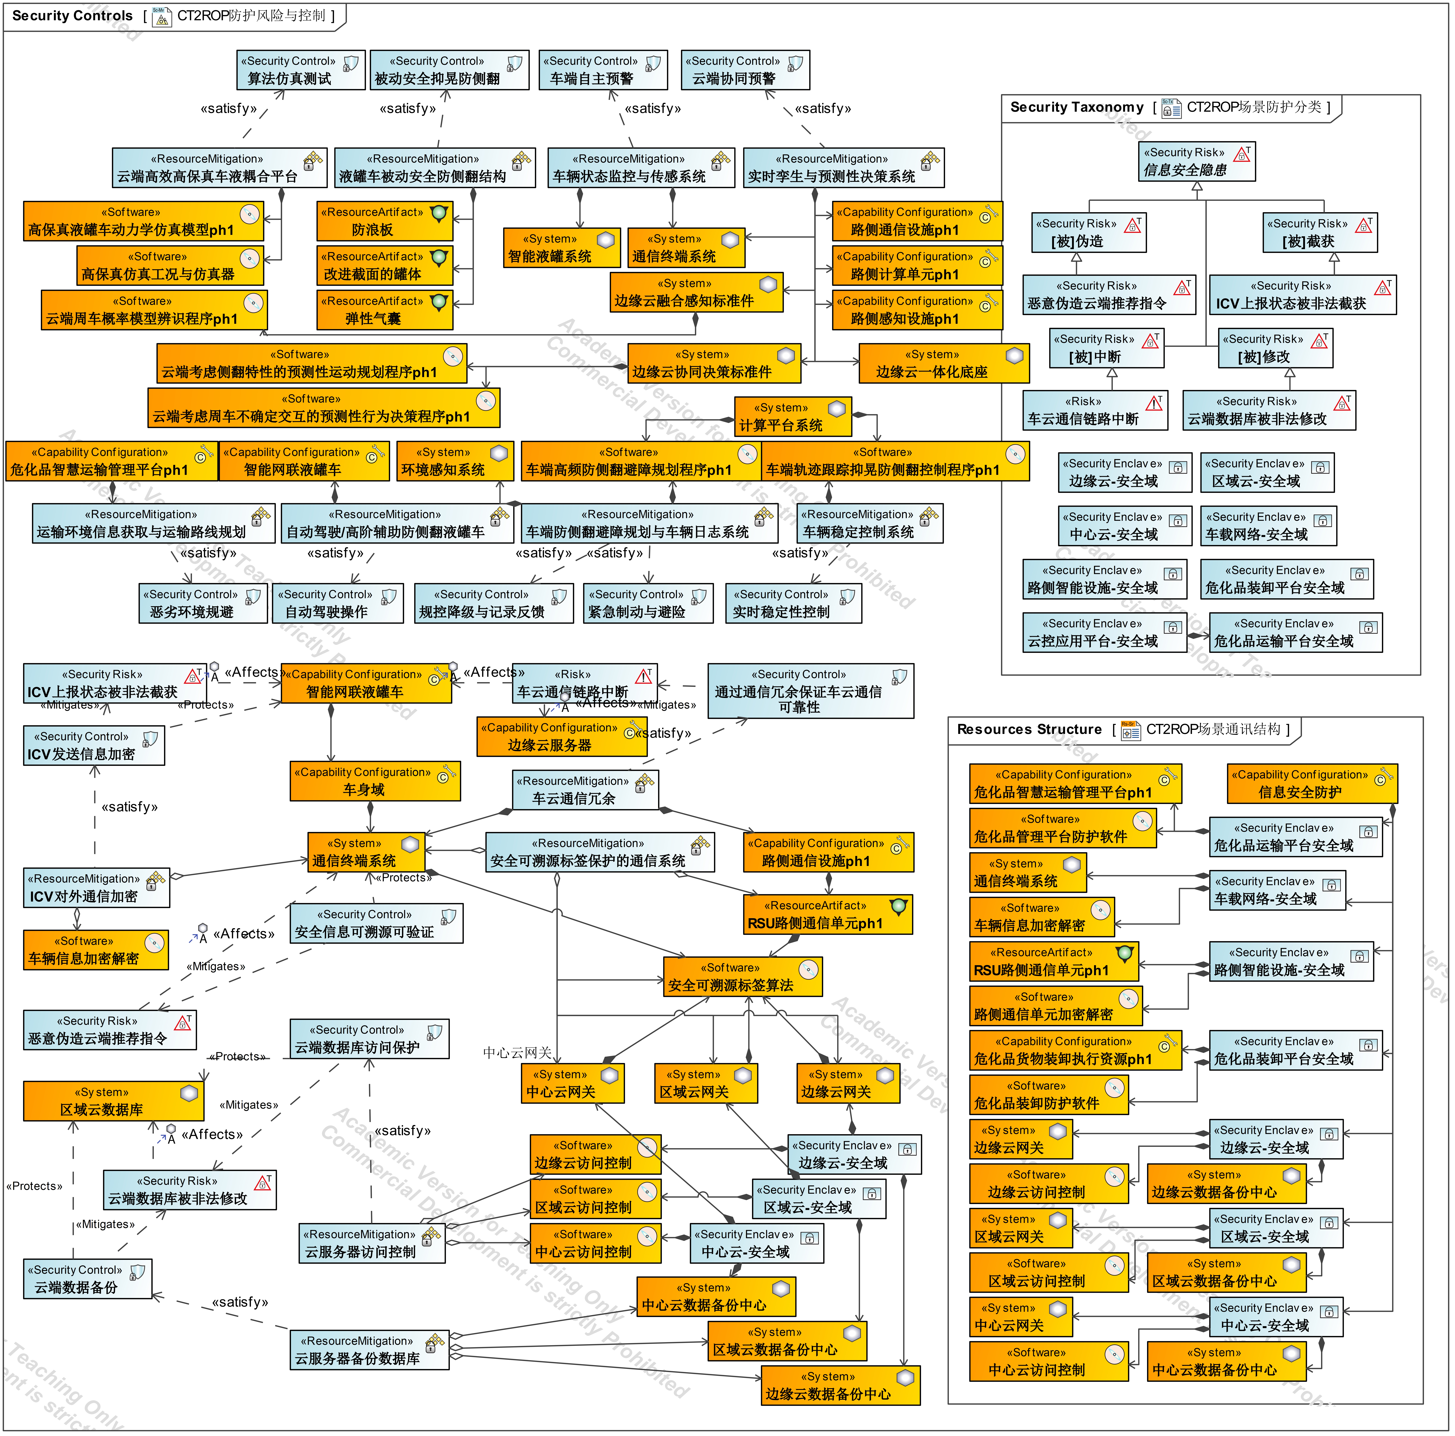
\includegraphics[width=1.0\linewidth]{fig/chap2/safe_resource.png}}
        \caption{CT2ROP场景安全与防护资源分析}
        \label{fig:safety_model}
      \end{figure}

      资源阶段据此进一步落实了服务层结论：云端算法设计建立在可支撑交通孪生、周车预测和长时域推演的资源条件之上，车端算法设计建立在独立可运行的感知、规划与控制资源之上，后续场景仿真则由战略环境参数与资源性能参数共同驱动。本阶段完成了从体系架构到后续章节算法实现与场景验证间的参数贯通。


\section{本章小结}

本章围绕车云协同液罐车防侧翻任务，首先分析了IVCPS的体系属性及其对建模方法的要求，指出IVCPS具有场景任务并发、资源共享和持续演进等特征，因此需要采用面向场景任务、能够支持闭环验证的分场景基于模型与仿真的体系工程方法开展架构建模。

在此基础上，本文构建了CT2ROP场景任务体系架构，并从战略、运行、服务和资源四个阶段对其进行了分析。战略分析明确了低渗透率条件下CT2ROP的阶段定位、风险分层与核心能力；运行分析明确了车端、云端、路侧及相关平台之间的运行分工；服务分析给出了场景特有服务及其约束，并通过服务参数仿真得出了保证稳定性与响应时效性的参数设置等关键结论；资源分析进一步落实了支撑主动安全能力的关键资源，并完成了从架构到后续场景仿真的参数贯通。CT2ROP架构结果向后续方法设计的约束传递关系如图~\ref{fig:arch_method_mapping_v3}所示。

\begin{figure}[htbp]
    \centering
    {
      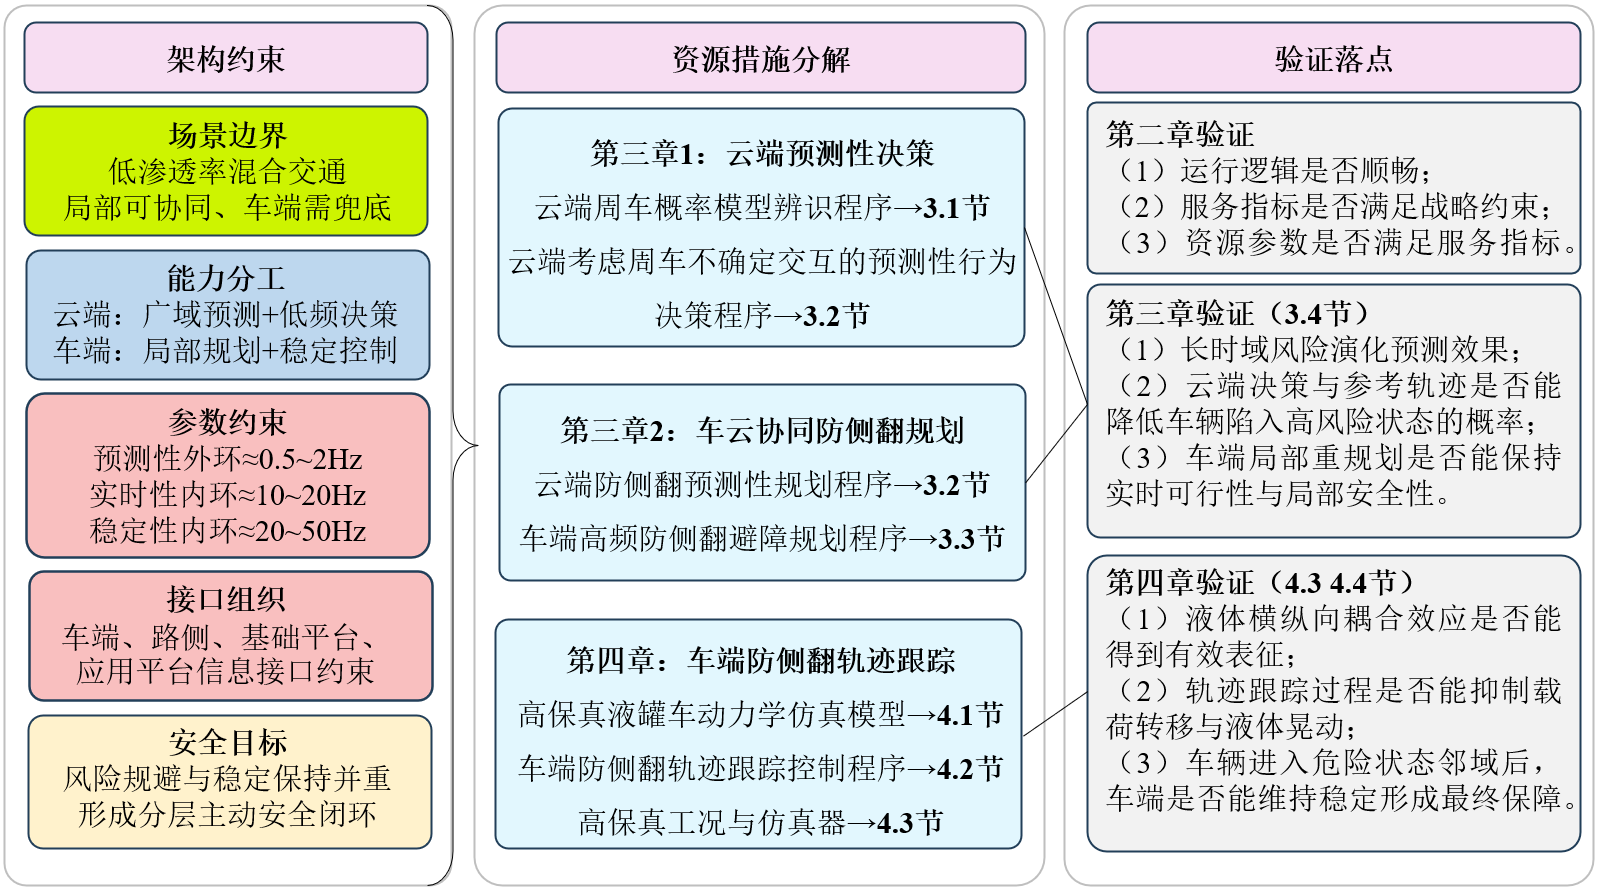
\includegraphics[width=1.0\linewidth]{fig/chap2/arch_method_mapping_v3.png}
    }
    \caption{CT2ROP架构结果向后续方法设计的约束传递关系}
    \label{fig:arch_method_mapping_v3}
\end{figure}

本章在此基础上，对前述分析结果作进一步归并，并据此梳理第三章云端预测性决策与车云协同防侧翻规划、第四章车端轨迹跟踪抑晃防侧翻控制之间的层次关系、功能分工与验证落点。

本章架构分析形成了五类对后续研究具有直接指导意义的设计约束，即场景边界约束、能力分工约束、参数指标约束、接口组织约束与安全目标约束。具体而言，场景边界约束给出了低渗透率、混合交通、局部可协同和车端需兜底的应用环境定义；能力分工约束明确了云控基础平台、危化品运输调度平台、智能网联液罐车端和路侧设施的任务边界；时间尺度等参数约束给出了云端外环、车端规划层与车端控制层在更新频率上的层级划分；接口组织约束明确了车、路、云及相关平台在场景任务中的协同关系；安全目标约束统一规定了后续方法设计需要同时服务于风险规避与稳定保持两个层级。

通过本章分析，本文最终形成了“云端低频预测、车端中频规划、车端高频控制”的车云协同液罐车防侧翻分层决控架构，并明确了云端与车端的功能边界、服务接口、时延约束和降级关系。这些结论为后续章节中云端预测性决策规划方法、车端防侧翻跟踪控制方法以及实验验证方案的设计提供了体系架构依据。
